\chapter{\label{chap:desenvolvimento}Desenvolvimento}

O desenvolvimento do sistema pode ser dividido em duas partes: i) o desenvolvimento da ontologia de cardápio e ii) o desenvolvimento da aplicação móvel para Android. Primeiramente, foi desenvolvida a estrutura da ontologia para, posteriormente, integrá-la à aplicação. A seguir, será apresentado o desenvolvimento de ambas as partes do sistema, bem como as modificações realizadas a partir da proposta inicial da aplicação e as dificuldades encontradas durante a evolução do projeto.

\section{\label{sec:ontologia}Ontologia de Cardápio}

Apesar de haver algumas ontologias de comida ou restaurantes já desenvolvidas, optou-se pela criação de uma ontologia própria que condizesse com o escopo do trabalho. Para a construção desta ontologia para cardápios, foram usadas como base outras ontologias relacionadas a comidas. A principal influência foi uma ontologia de pizza desenvolvida pela universidade de Stanford\footnote{http://protege.stanford.edu/ontologies/pizza/pizza.owl}, uma vez que um cardápio é composto por diversos produtos que apresentam atributos semelhantes aos de uma pizza. Voltaremos a falar desses atributos nos próximos parágrafos.

A estrutura da ontologia é dividida em duas partições iniciais: \emph{Partição Domínio} e \emph{Partição Valor}. Dentro da partição de domínio, encontram-se os \emph{produtos} e os \emph{ingredientes}, os quais serão atribuídos aos produtos do cardápio. Os produtos da aplicação referem-se aos produtos do cardápio em si e é dentro desta classe que as informações essenciais a nossa aplicação estão armazenadas. Cada produto apresenta ou herda as seguintes propriedades:
\begin{itemize}
	\item Ingredientes;
	\item Preço;
	\item Restrições alimentares:
	\begin{itemize}
		\item Se possui glúten;
		\item Se possui lactose;
		\item Se é vegetariano;
		\item Nível de sal;
		\item Nível de gordura;
	\end{itemize}
	\item Se é um produto contável ou não.
\end{itemize}

Já a partição de valor é composta pelas classes \emph{Gorduras} e \emph{Nível de Sal}, representando todas as propriedades que podem ser compostas por uma gradação de valores. Cada uma dessas classes apresentam, por sua vez, três subclasses que condizem à intensidade destas propriedades em um produto. Desta forma, o nível de sal de uma determinada comida pode ser indicado com um dos três níveis criados na ontologia, sendo eles: \emph{pouco salgado}, \emph{meio salgado} e \emph{salgado}. Para a indicação desta propriedade no produto, criou-se a propriedade \emph{temSal}, cujo domínio é uma classe do tipo Produto e o contradomínio é uma classe do tipo Nível de Sal. 

Para gerar relações entre classes e propriedades, foram criadas \emph{propriedades de objeto} e \emph{propriedades de dados}. As propriedades de objeto são utilizadas quando tanto o domínio quanto o contradomínio da expressão são classes da ontologia; já as propriedades de dados aplicam-se quando o contradomínio é composto por um tipo de dado, como um \emph{value} ou um \emph{boolean}. Algumas propriedades e suas relações com as classes são demonstradas a seguir, na Figura \ref{fig:propriedades}.
\begin{figure}
	\centering
	\caption[Propriedades da Ontologia]{Exemplos de propriedades da ontologia}
	\label{fig:propriedades}
	\subfigure[c][Propriedade \emph{temIngrediente}. Seu domínio são as classes \emph{Comida} ou \emph{Bebida} e o contradomínio é \emph{Ingrediente}]
	{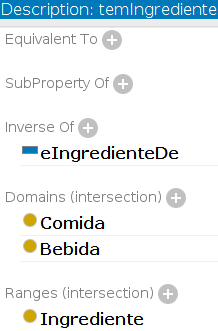
\includegraphics[width=0.3\textwidth]{./fig/propriedade-1.png}}
	\qquad
	\subfigure[c][Propriedade \emph{preco}. Seu domínio é a classe \emph{Produto} e o contradomínio é um valor do tipo \emph{double}]
	{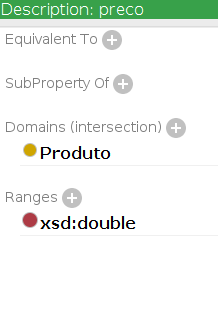
\includegraphics[width=0.3\textwidth]{./fig/propriedade-2.png}}
\end{figure}

\section{Integração da Ontologia com a Aplicação}

Sendo Java a linguagem de programação utilizada no desenvolvimento da aplicação, buscou-se uma API que fosse compatível com a linguagem e que consultasse a ontologia de forma eficiente. A princípio, a interface escolhida fora a OWL API\footnote{http://owlapi.sourceforge.net/}, uma interface para criação, manipulação e serialização de ontologias OWL. Todavia, apesar de ser desenvolvida para a linguagem Java, essa API não se apresentou compatível com o ambiente Android, sendo assim necessária uma nova busca, resultando na descoberta do \emph{framework} Apache Jena. Jena é uma ferramenta para a construção de aplicações que utilizam web semântica ou dados conectados (\emph{linked data}) e é responsável pelo controle de APIs de diversas estruturas de dados, como ontologias, Resource Description Framework (RDF), SPARQL, entre outras. Este \emph{framework} possui uma versão compatível com o ambiente Android, o AndroJena\footnote{https://github.com/lencinhaus/androjena} e, por isso, foi escolhida para realizar integração entre a ontologia e a aplicação do sistema.

A integração da ontologia para a aplicação torna-se necessária uma vez que é a partir dela que os produtos do cardápio serão apresentados ao usuário. Um produto, ou uma categoria de produtos, deve apresentar todas as propriedades citadas na seção \ref{sec:ontologia}, possibilitando, assim, a sua catalogação. Entretanto, algumas classes não apresentam certas características declaradas -- por exemplo, como mostrado na Figura \ref{fig:integracao-1}, o produto \emph{Pastel} não possui as características \emph{tem gordura, tem sal, lactose} e \emph{vegetariano}, porém suas classes sucessoras contêm tais informações. Isto se dá pelo fato de que as propriedades de uma classe estão dispostas na ontologia de forma esparsa; existem classes que herdam suas propriedades de \emph{forma anônima} ou aquelas que são muito abrangentes e, desta forma, ainda não dispõem de propriedades tão definidas. Por exemplo, a classe \emph{Pastel de Forno} tem pouca gordura e pouco sal (propriedades inerentes à classe); é contável, tem glúten e custa R\$5,50 (propriedades herdadas anonimamente da classe \emph{Pastel}); e, também, possui produtos com lactose e vegetarianos (propriedades de suas \emph{classes filhas}). Sendo assim, fora preciso transformar a representação do conhecimento de uma estrutura para a outra.

\begin{figure}[H]
		\centering
		\caption[Integração da Ontologia -- Passo 0]{Passo 0 -- Estrutura da ontologia antes da integração. Os textos à esquerda representam os atributos herdados de forma anônima e os textos à direita representam os atributos das classes}
		\label{fig:integracao-1}
		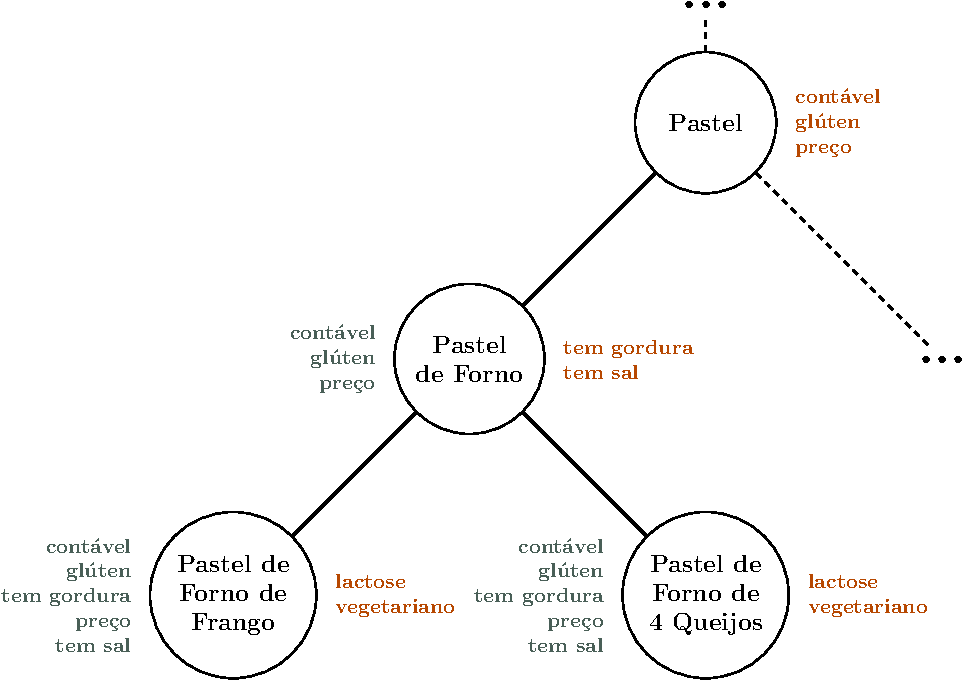
\includegraphics[width=0.6\linewidth]{./pdf/tikz/toptop-1.pdf}
\end{figure}

O processo de aquisição de todas as propriedades de um produto começou com o caminhamento do nodo raiz até os nodos folhas da árvore da ontologia. Observando a Figura \ref{fig:integracao-2}, é possível notar que algumas propriedades devem ser passadas para os nodos filhos durante o percorrimento de cima pra baixo:

\begin{figure}[H]
	\centering
	\caption[Integração da Ontologia -- Passos 1--4]{Passos 1--4 -- Os atributos das classes superiores são passados para suas filhas. Os textos à esquerda representam os atributos herdados de forma anônima e os textos à direita representam os atributos das classes}
	\label{fig:integracao-2}
	\subfigure[c][Passo 1 -- A classe \emph{Pastel de Forno} recebe os atributos da classe \emph{Pastel}]
	{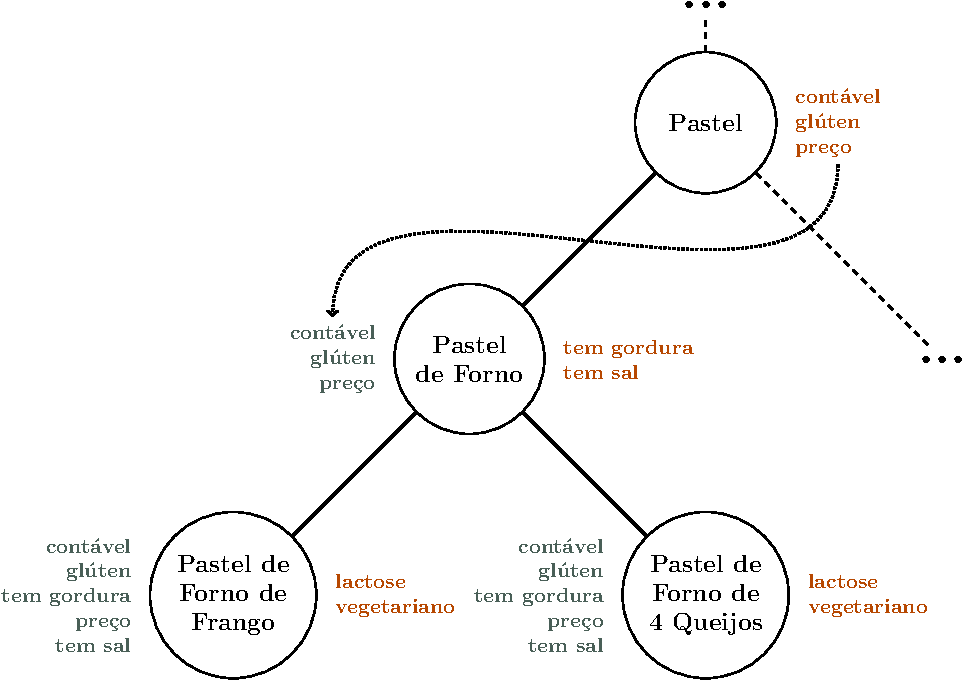
\includegraphics[width=0.45\textwidth]{./pdf/tikz/topdown-1.pdf}}
	\qquad
	\subfigure[c][Passo 2 -- Os atributos recebidos são armazenados em sua própria lista de atributos]
	{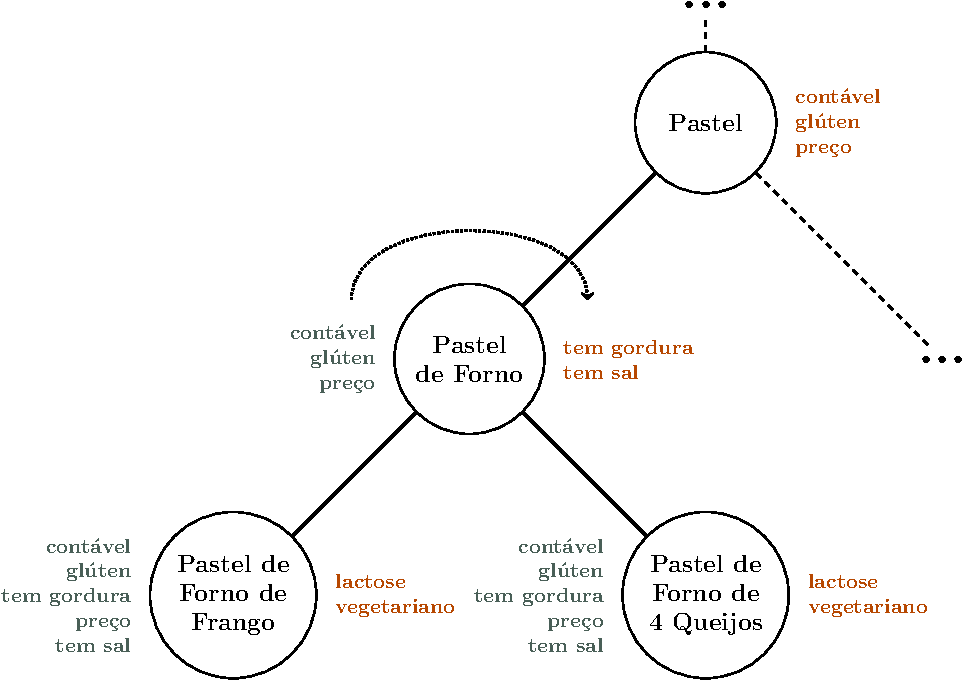
\includegraphics[width=0.45\textwidth]{./pdf/tikz/topdown-2.pdf}}
	\qquad
	\subfigure[c][Passo 3 -- O mesmo processo se repete, agora com a classe \emph{Pastel de Forno}]
	{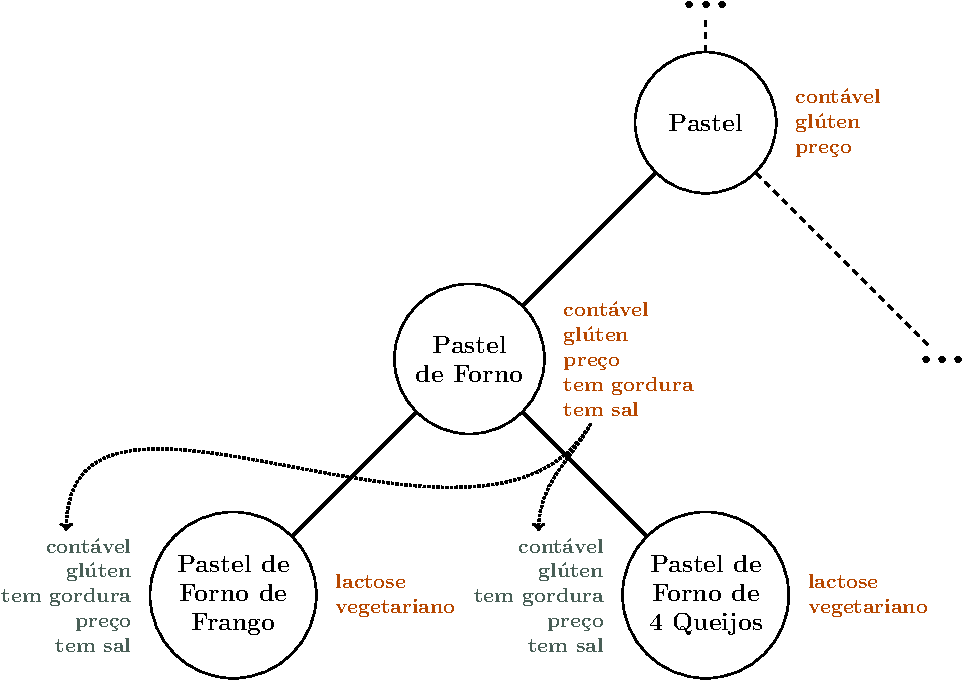
\includegraphics[width=0.45\textwidth]{./pdf/tikz/topdown-3.pdf}}
	\qquad
	\subfigure[c][Passo 4 -- Os atributos recebidos são armazenados em sua própria lista de atributos]
	{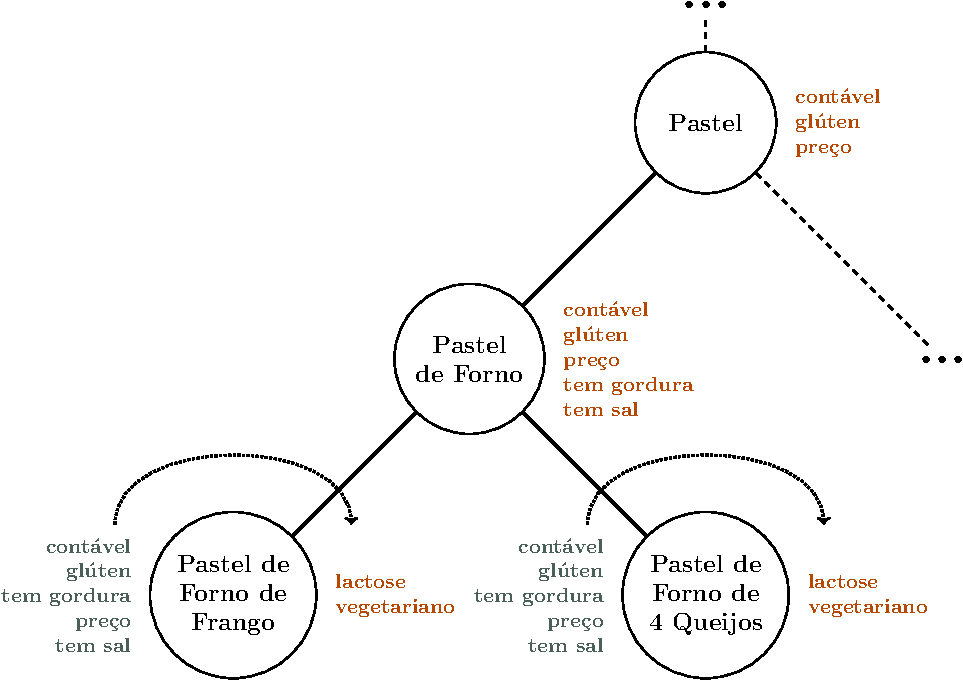
\includegraphics[width=0.45\textwidth]{./pdf/tikz/topdown-4.pdf}}
\end{figure}

Esse processo de propagação de características é feito com o uso de uma estrutura de dados HashMap, a qual armazena as propriedades do nodo atual e seus valores (verdadeiro ou falso) e propaga estes dados para seus nodos filhos. Desta forma, ao chegar em um nodo folha, seu mapa de propriedades deve estar totalmente preenchido, como mostrado na Figura \ref{fig:integracao-3}:

\begin{figure}[H]
	\centering
	\caption[Integração da Ontologia -- Passo 5]{Passo 5 -- Todos os atributos foram transferidos às classes sucessoras. Os textos à esquerda representam os atributos herdados de forma anônima e os textos à direita representam os atributos das classes}
	\label{fig:integracao-3}
	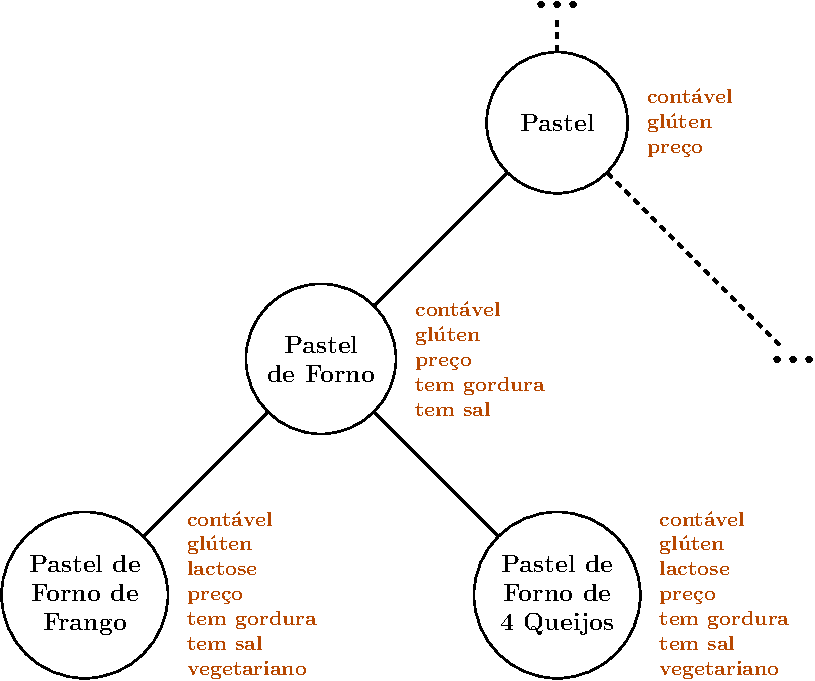
\includegraphics[width=0.55\linewidth]{./pdf/tikz/topdown-5.pdf}
\end{figure}

Nota-se que, apesar dos nodos folhas possuírem todos os valores de suas propriedades, o mesmo não ocorre com as classes mais gerais. Sendo assim, torna-se necessário um novo caminhamento, desta vez do nodo folha ao nodo raiz, buscando atribuir aos primeiros nodos as características que estão presentes em seus filhos. Para isso, foi desenvolvido um critério de atribuição de valores, buscando armazenar apenas os valores que seriam relevantes à aplicação. Este processo é demonstrado na Figura \ref{fig:integracao-4}. 

\begin{figure}[H]
	\centering
	\caption[Integração da Ontologia -- Passos 6--10]{Passos 6--10 -- Os atributos são repassados das folhas à raiz}
	\label{fig:integracao-4}
	\subfigure[c][Passo 6 -- União entre os atributos das classes folhas e os de sua classe mãe]
	{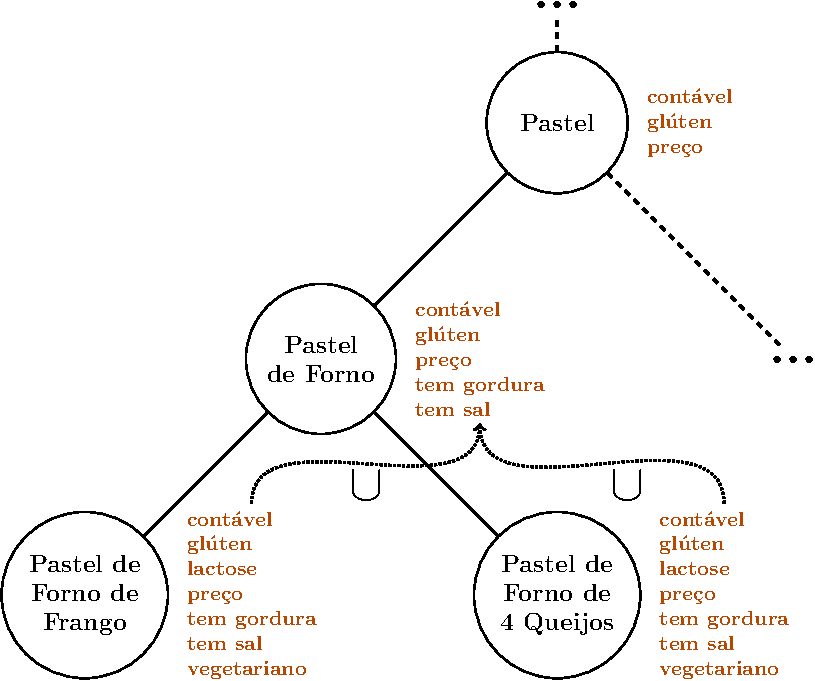
\includegraphics[width=0.45\textwidth]{./pdf/tikz/bottomup-1.pdf}}
	\qquad
	\subfigure[c][Passo 7 -- Classe \emph{Pastel de Forno} agora possui os atributos de suas filhas]
	{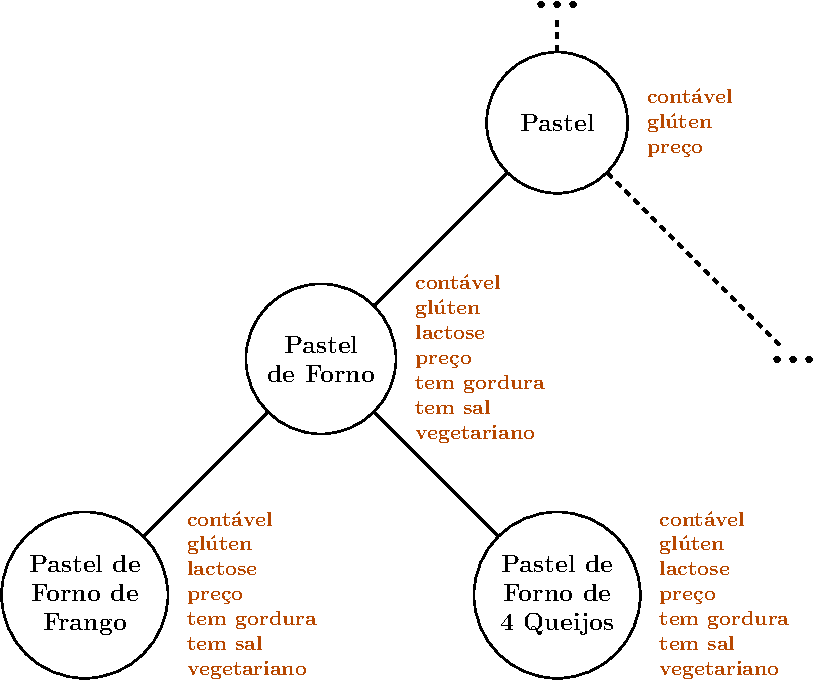
\includegraphics[width=0.45\textwidth]{./pdf/tikz/bottomup-2.pdf}}
	\qquad
	\subfigure[c][Passo 8 -- Classe \emph{Pastel de Forno} propaga estas informações a sua classe mãe]
	{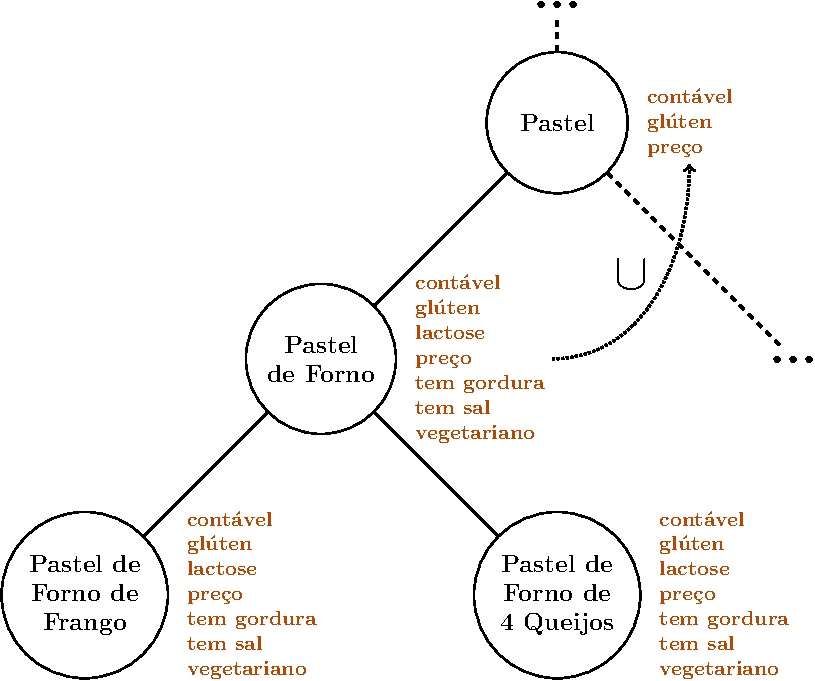
\includegraphics[width=0.45\textwidth]{./pdf/tikz/bottomup-3.pdf}}
	\qquad
	\subfigure[c][Passo 9 -- Classe \emph{Pastel} agora possui os atributos de suas filhas]
	{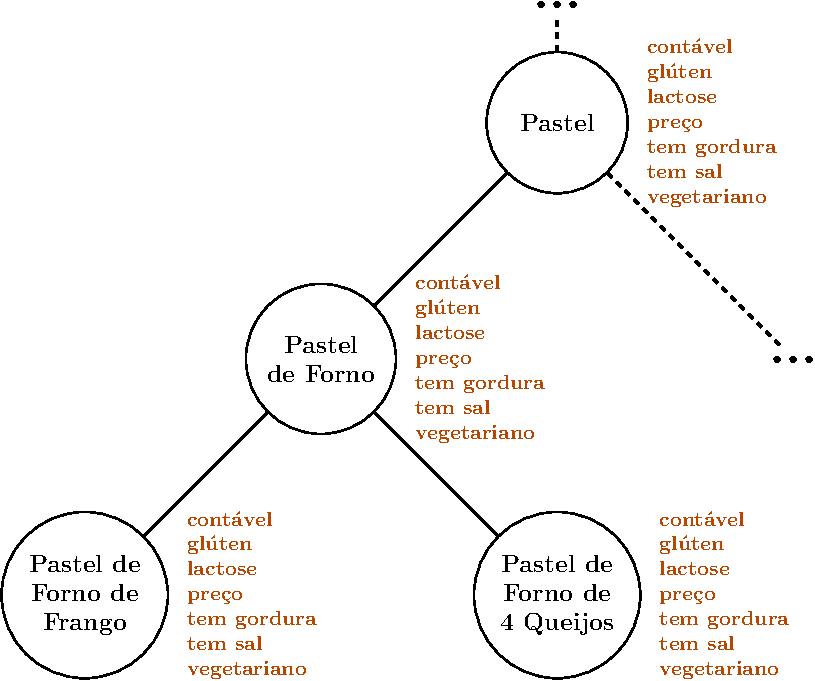
\includegraphics[width=0.45\textwidth]{./pdf/tikz/bottomup-4.pdf}}
	\qquad
	\subfigure[c][Passo 10 -- Classe \emph{Pastel} propaga estas informações para suas classes superiores]
	{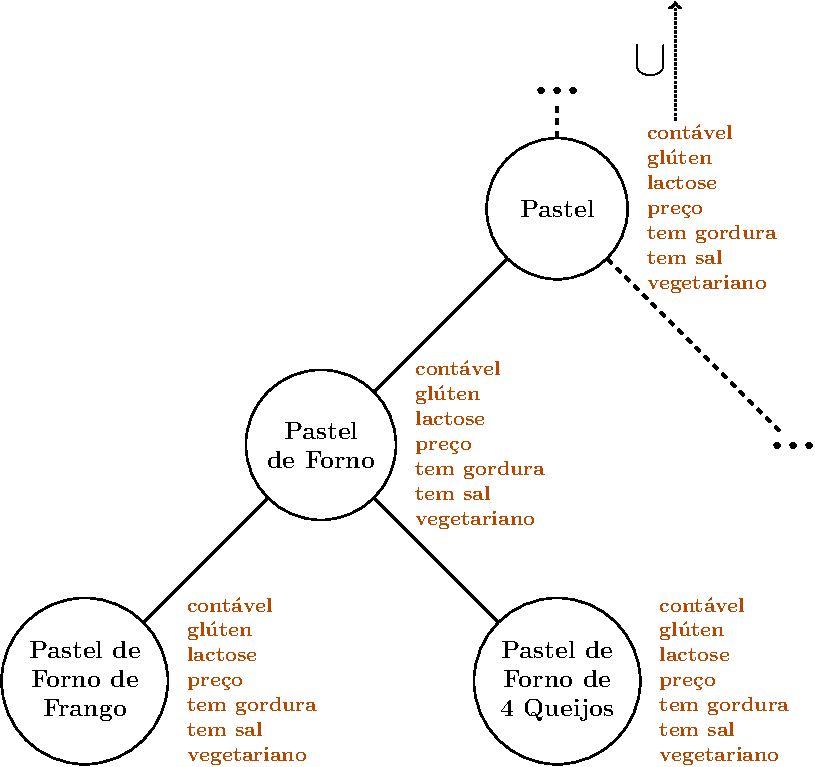
\includegraphics[width=0.45\textwidth]{./pdf/tikz/bottomup-5.pdf}}
\end{figure}

\section{Aplicação}

Sendo possível o acesso à ontologia através da aplicação, bastou incorporar os demais elementos. Primeiramente, a aplicação apresenta uma tela inicial (Figura \ref{fig:cardapio-virtual-1}(a)), com a listagem dos todos os restaurantes armazenados no sistema e dos restaurantes favoritos do usuário, uma barra de busca e um botão para a tela de ajuda. Ao clicar no botão de busca, a barra se expande, exibindo o campo de busca com suas opções de pesquisa, as quais vão sendo alteradas à medida que o usuário insere caracteres neste campo. Além de busca por digitação, existe, também, a opção de procurar um restaurante através do modo de busca por voz (Figura \ref{fig:cardapio-virtual-1}(b)).

\begin{figure}[H]
	\centering
	\caption[Telas da Aplicação 1--3]{Tela inicial da aplicação e seu sistema de buscas}
	\label{fig:cardapio-virtual-1}
	\subfigure[c][Tela inicial da aplicação]
	{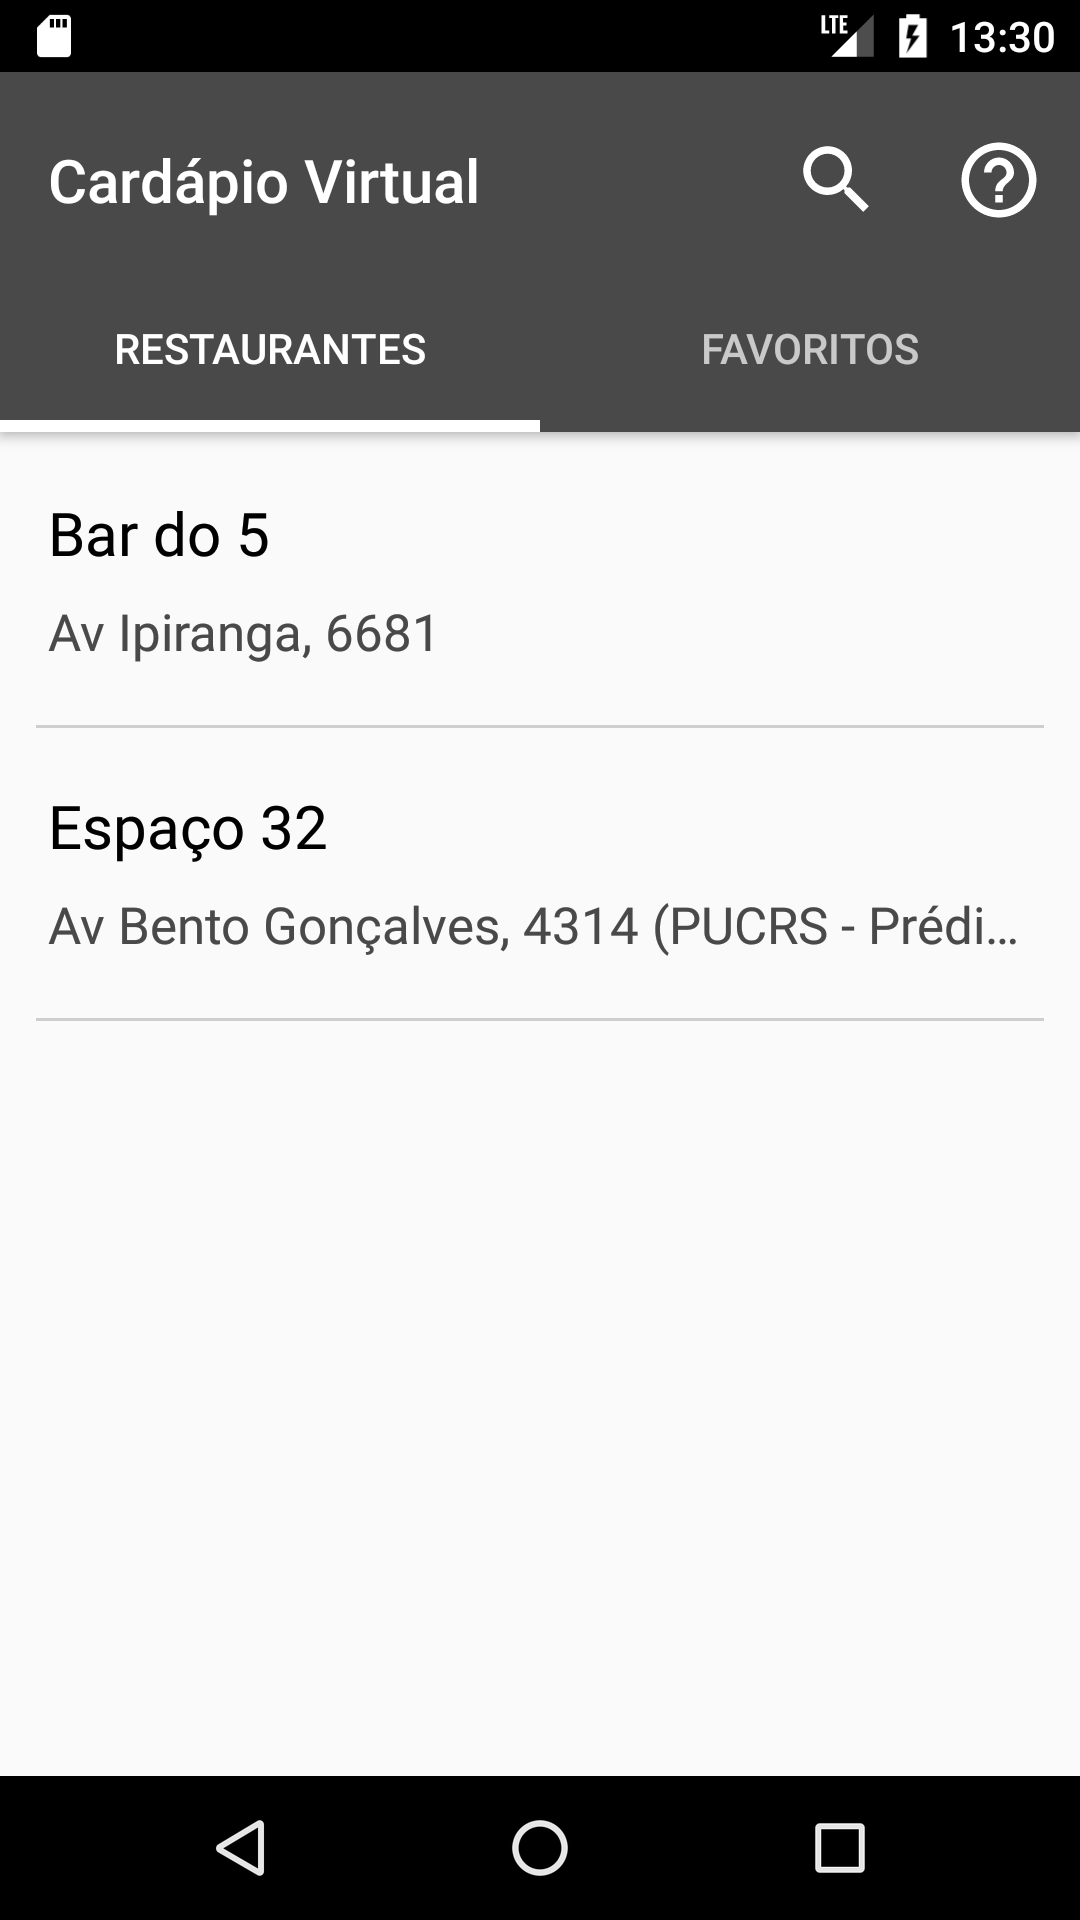
\includegraphics[width=0.29\textwidth]{./fig/cardapio-virtual/tela-inicial-1.png}}
	\qquad
	\subfigure[c][Barra de buscas de restaurantes]
	{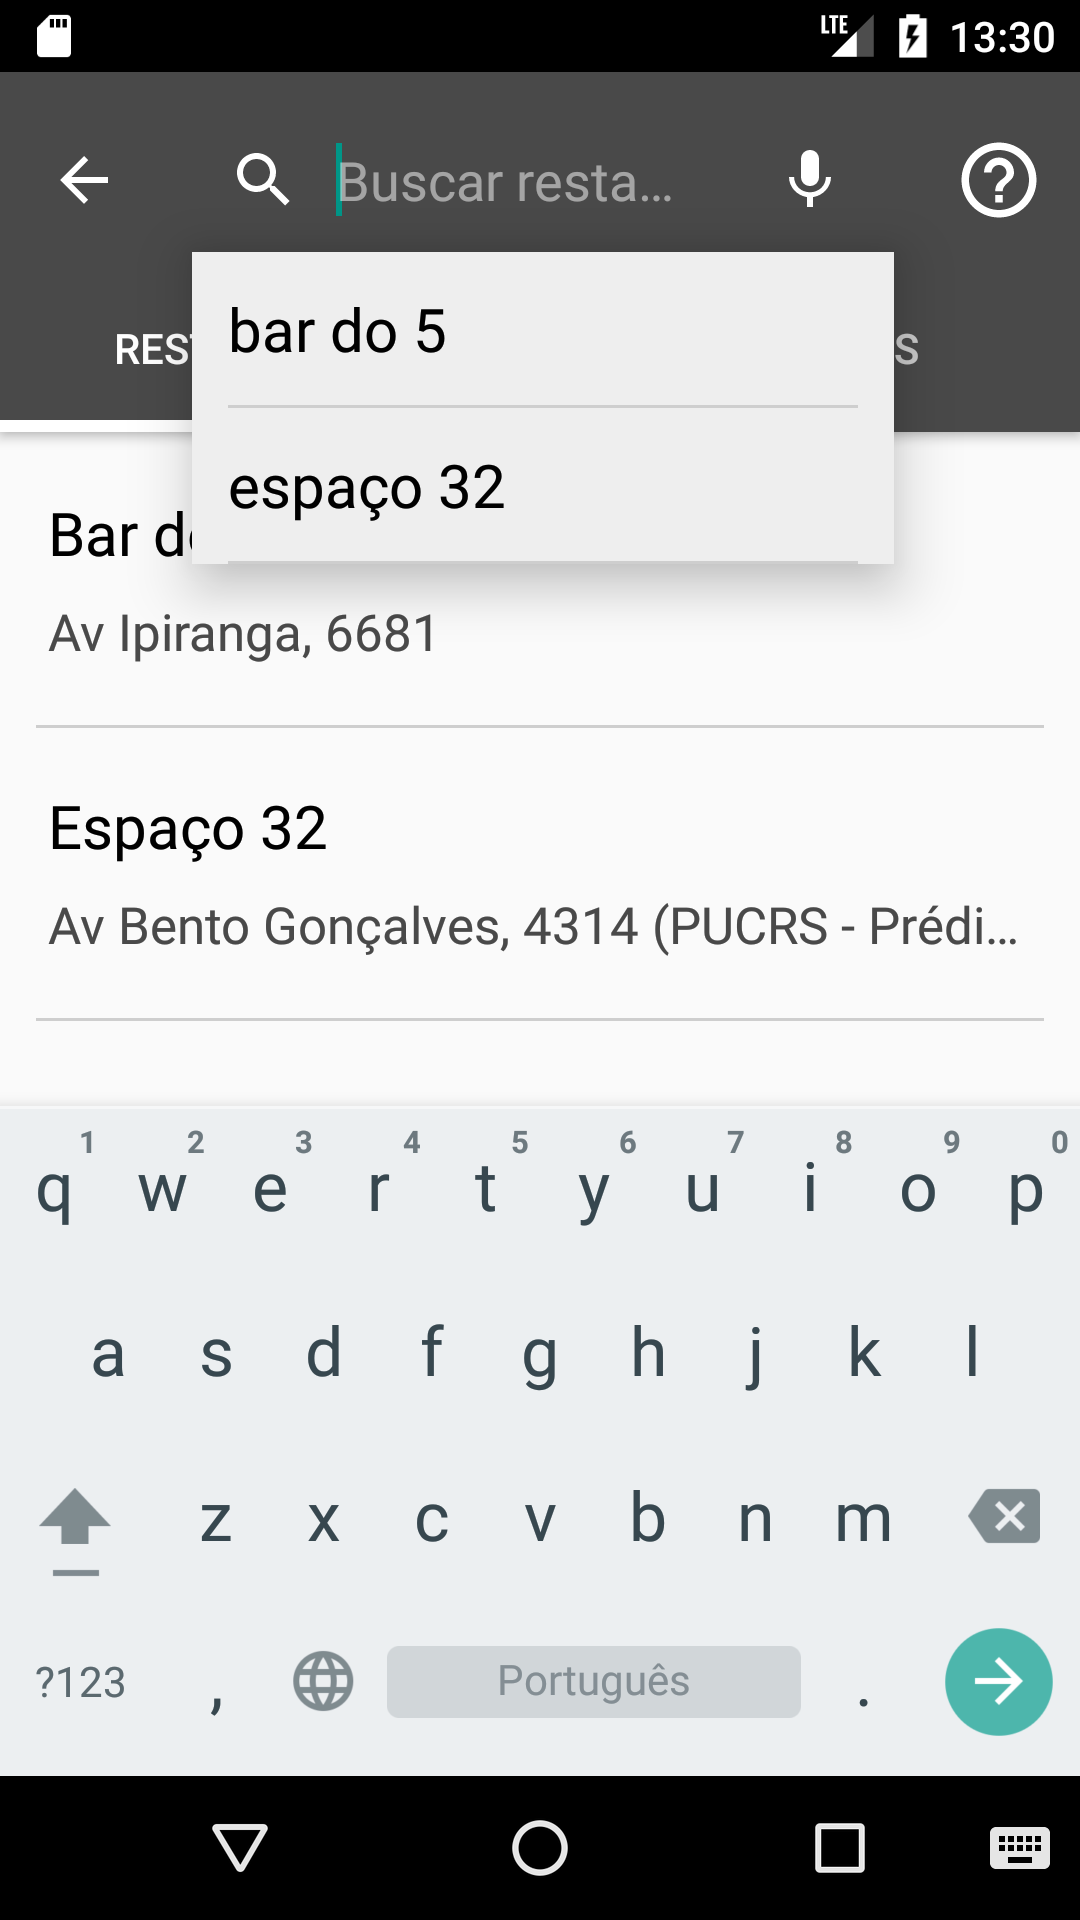
\includegraphics[width=0.29\textwidth]{./fig/cardapio-virtual/tela-inicial-2-busca.png}}
	\qquad
	\subfigure[c][Resultado da busca por "es"\ no sistema]
	{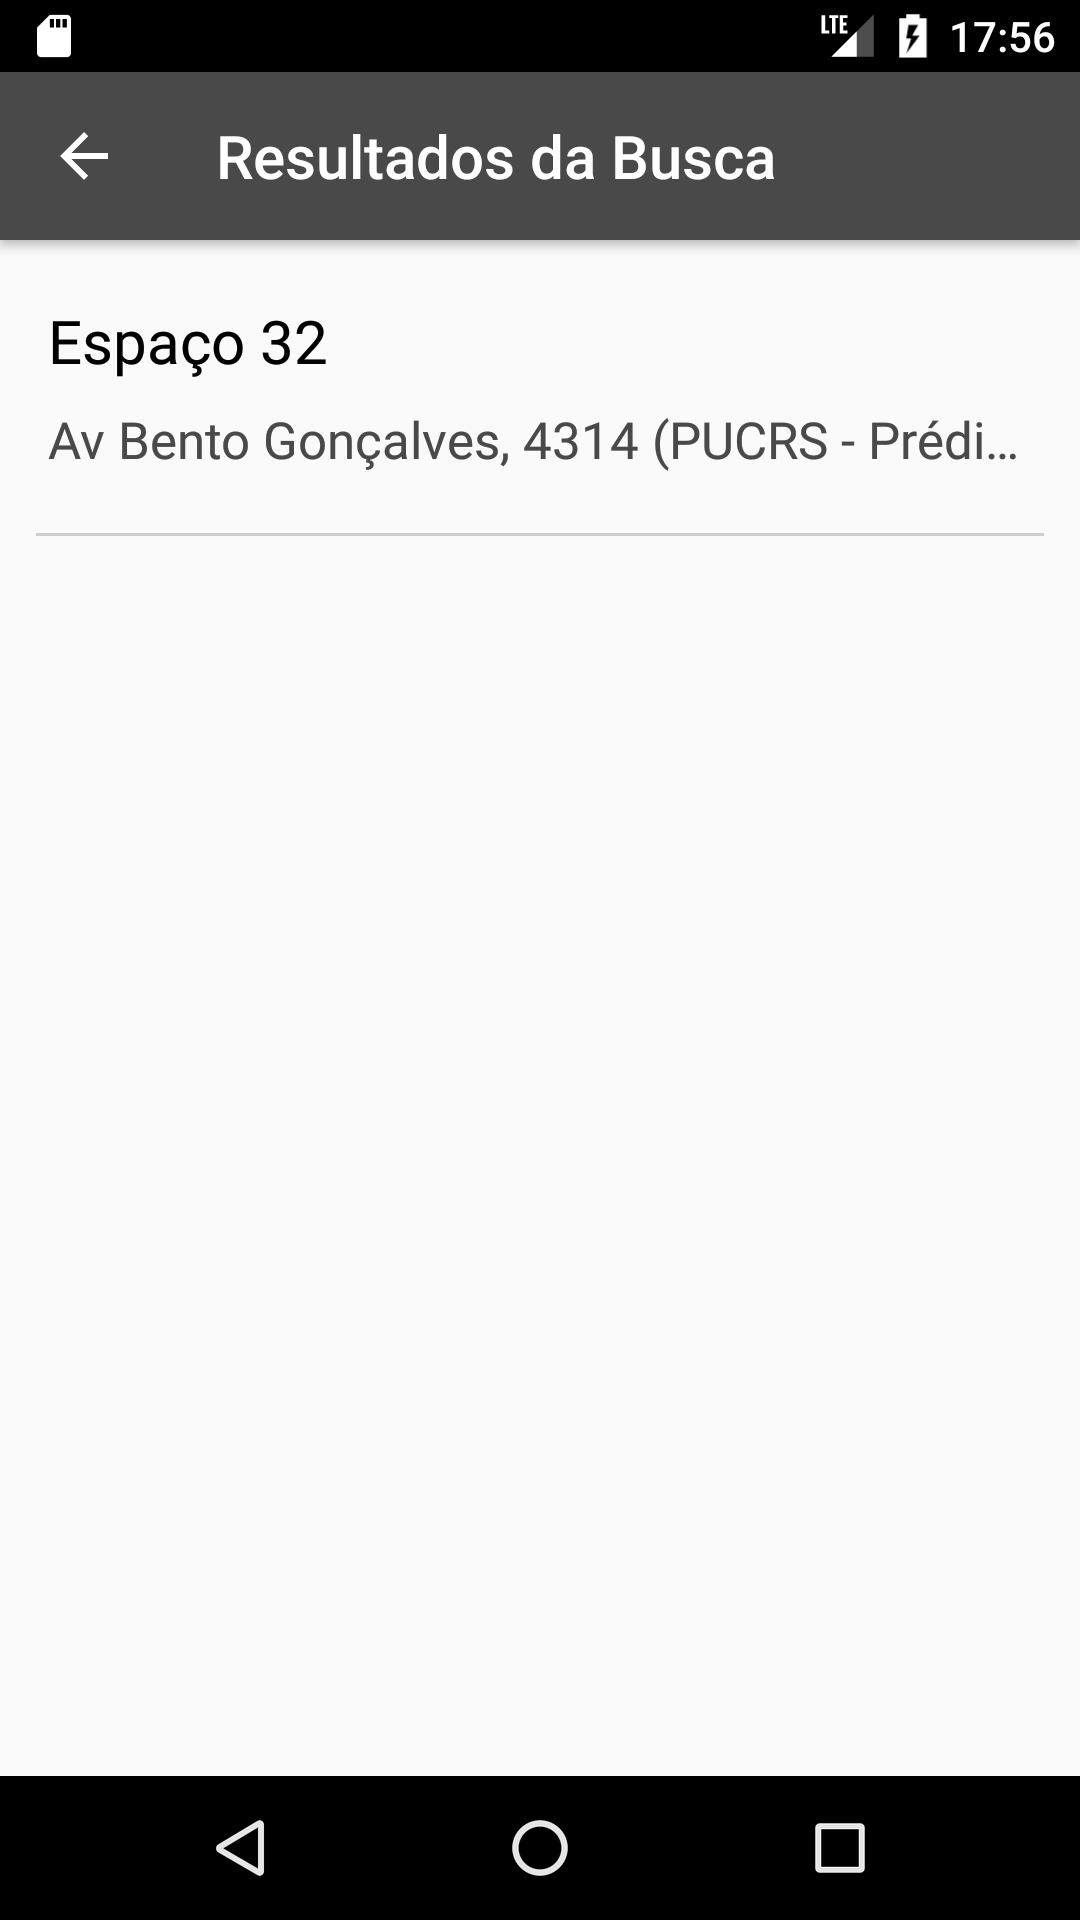
\includegraphics[width=0.29\textwidth]{./fig/cardapio-virtual/tela-busca.png}}
\end{figure}

A partir da tela principal (Figura \ref{fig:cardapio-virtual-1}(a)), o usuário é capaz de:
\begin{itemize}
	\item Selecionar um restaurante e acessar suas informações adicionais;
	\item Fazer uma busca e selecionar um dos restaurantes sugeridos pela barra de pesquisa, sendo levado para a tela de informações adicionais do local;
	\item Fazer uma busca e ir para a tela de resultado de buscas; e
	\item Acessar a tela de ajuda.
\end{itemize}
A tela de resultado da busca (Figura \ref{fig:cardapio-virtual-1}(c)) apenas lista os resultados que se encaixam com a pesquisa, possibilitando que o usuário selecione um dos locais ou volte para a tela inicial. A tela de informações adicionais de um restaurante, mostrada na Figura \ref{fig:cardapio-virtual-2}(a), apresenta uma breve descrição do local; suas informações básicas, como telefone e e-mail; acesso ao seu cardápio e um botão que possibilita ao usuário favoritar ou desfavoritar o local. Por fim, a tela de ajuda, apresentada na Figura \ref{fig:cardapio-virtual-2}(b)), exibe algumas perguntas e respostas que visam auxiliar o usuário durante sua experiência com a aplicação.

\begin{figure}[H]
	\centering
	\caption[Telas da Aplicação 4--5]{Telas de informações adicionais dos restaurantes e sistema de ajuda}
	\label{fig:cardapio-virtual-2}
	\subfigure[c][Tela de informações adicionais do restaurante Espaço 32]
	{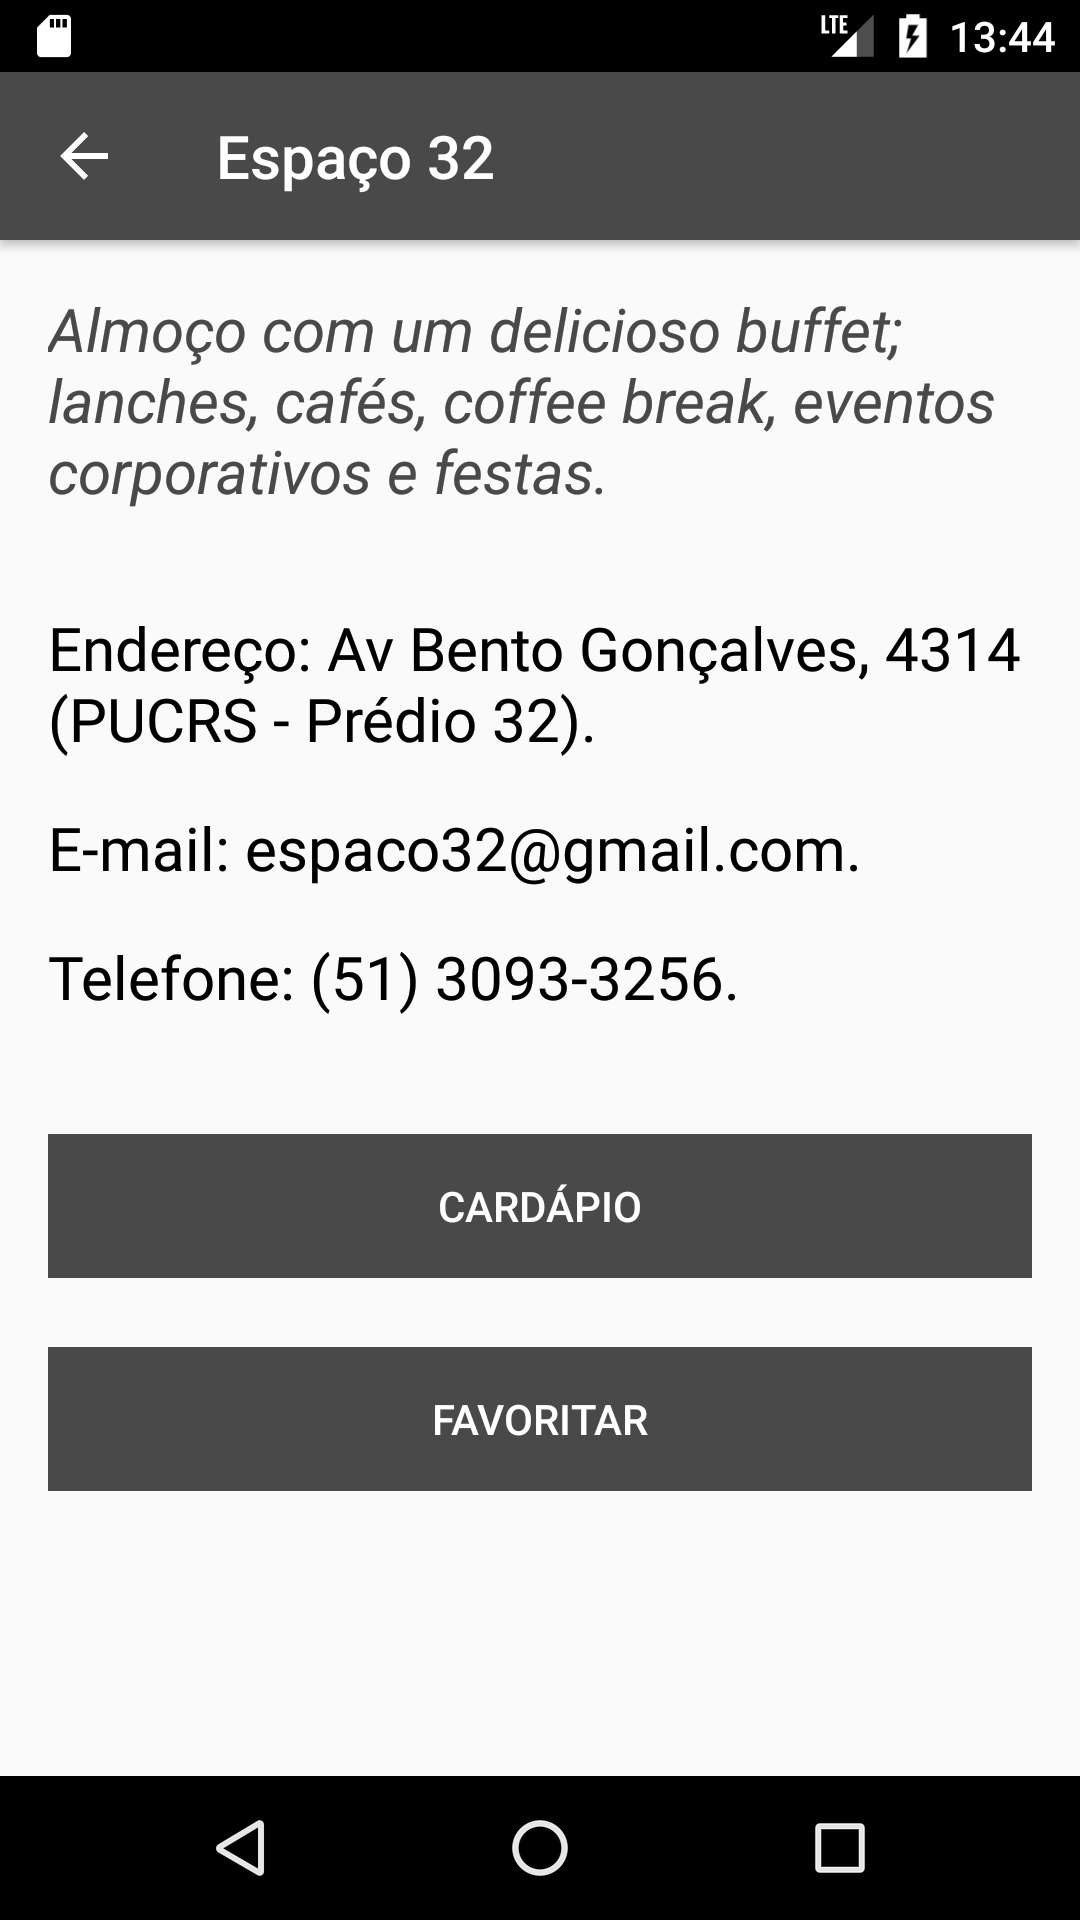
\includegraphics[width=0.3\textwidth]{./fig/cardapio-virtual/info-restaurante-1.png}}
	\qquad
	\subfigure[c][Tela de ajuda]
	{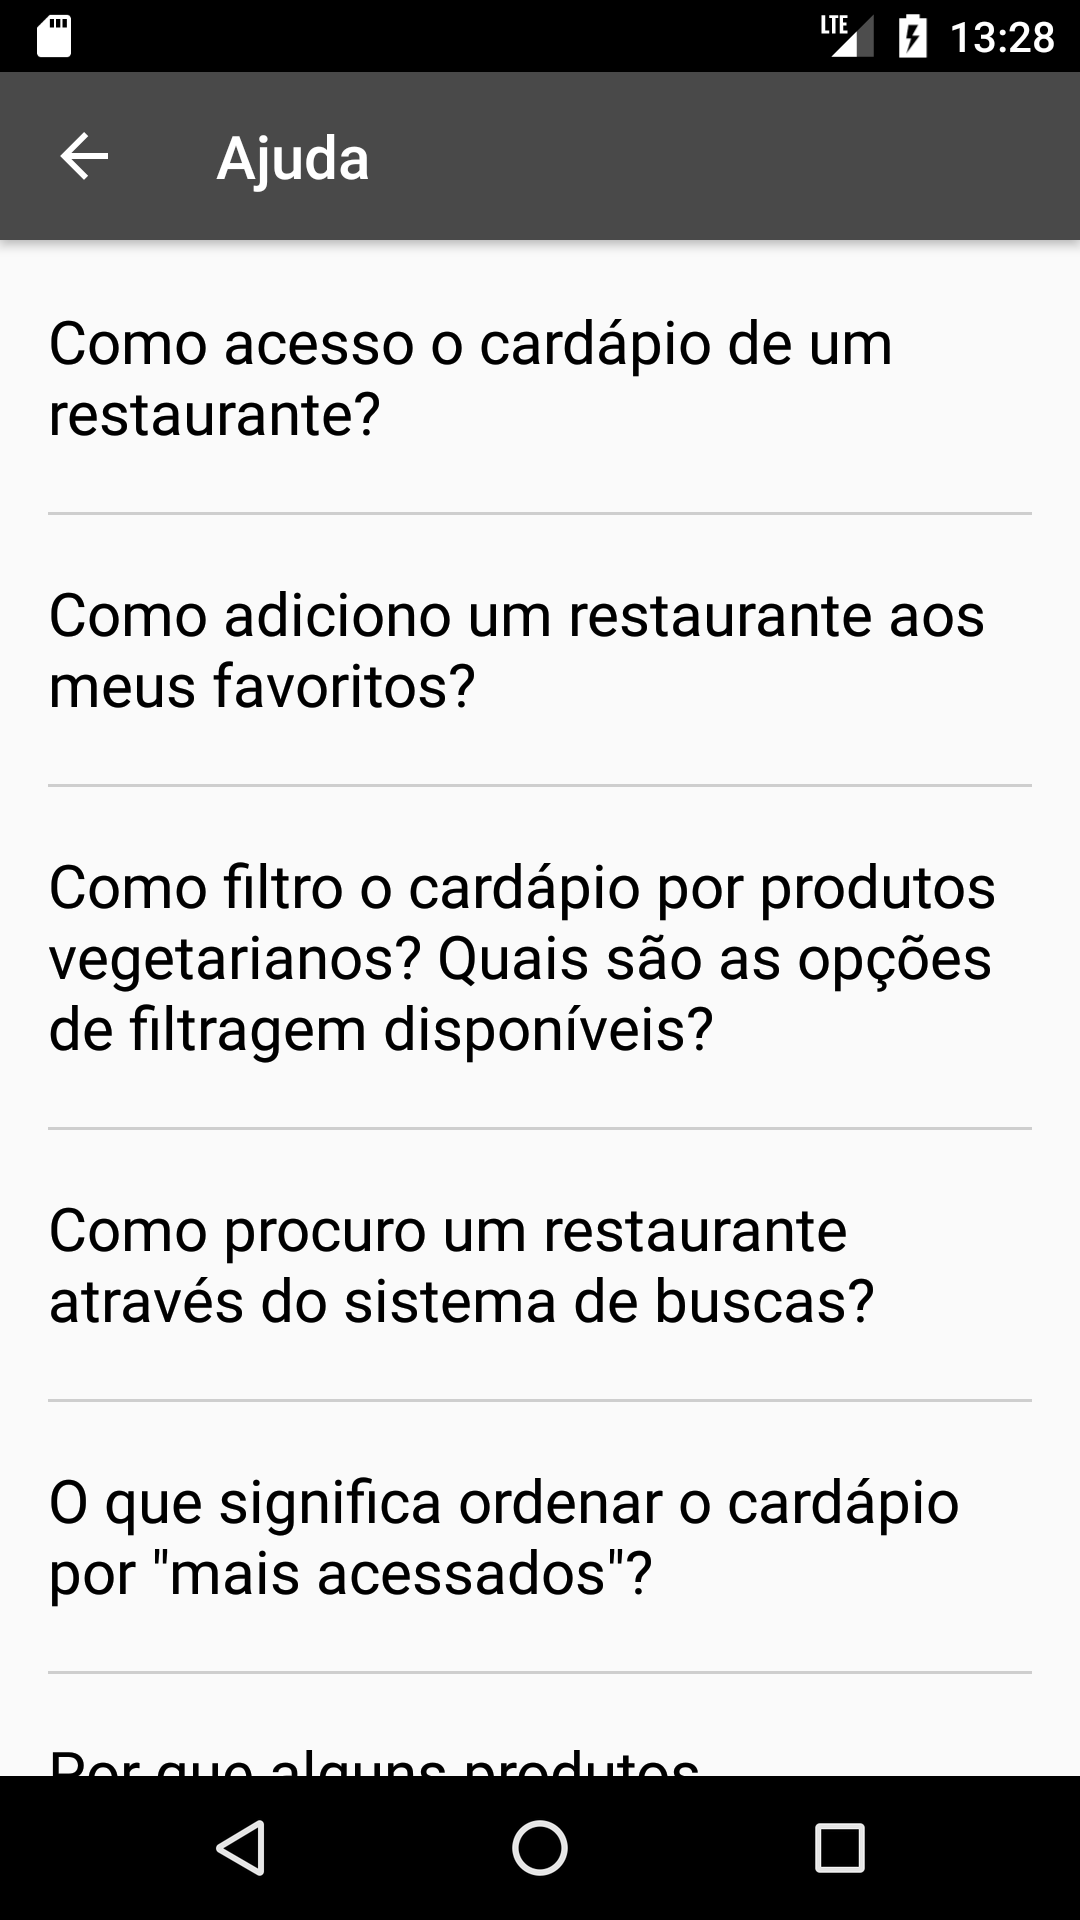
\includegraphics[width=0.3\textwidth]{./fig/cardapio-virtual/ajuda-1.png}}
\end{figure}

Seguindo o fluxo da aplicação, a próxima tela a ser exibida é a tela do menu (Figura \ref{fig:cardapio-virtual-3}(a) e \ref{fig:cardapio-virtual-3}(b)), a qual é acionada quando o usuário seleciona o cardápio de um restaurante. Esta tela apresenta os produtos disponíveis no local agrupados por categorias. Há também dois métodos de disposição dos itens do cardápio: o método de filtragem e o de ordenação. O primeiro permite que o usuário filtre os produtos do cardápio a partir de um ou mais dos seguintes critérios: sem glúten, sem lactose, vegetarianos, com pouca gordura e com pouco sal. Já o segundo permite ao usuário que os produtos sejam dispostos em ordem alfabética ou em ordem de acesso -- permitindo, assim, que os produtos mais acessados sejam facilmente encontrados nas próximas consultas. Estes métodos são apresentados nas Figuras \ref{fig:cardapio-virtual-3}(c) e \ref{fig:cardapio-virtual-3}(d). Por fim, ao selecionar um produto da lista, suas informações adicionais, ou seja, seus ingredientes, seu preço e sua quantidade disponível no local são exibidas na tela, como demonstrado na Figura \ref{fig:cardapio-virtual-4}(e). Sendo assim, o usuário tem acesso aos produtos dos restaurantes, bem como as informações básicas que necessita para escolher qual produto mais lhe agrada.

\begin{figure}[H]
	\centering
	\caption[Telas da Aplicação 6--10]{Demais telas da aplicação}
	\label{fig:cardapio-virtual-3}
	\subfigure[c][Tela inicial do cardápio]
	{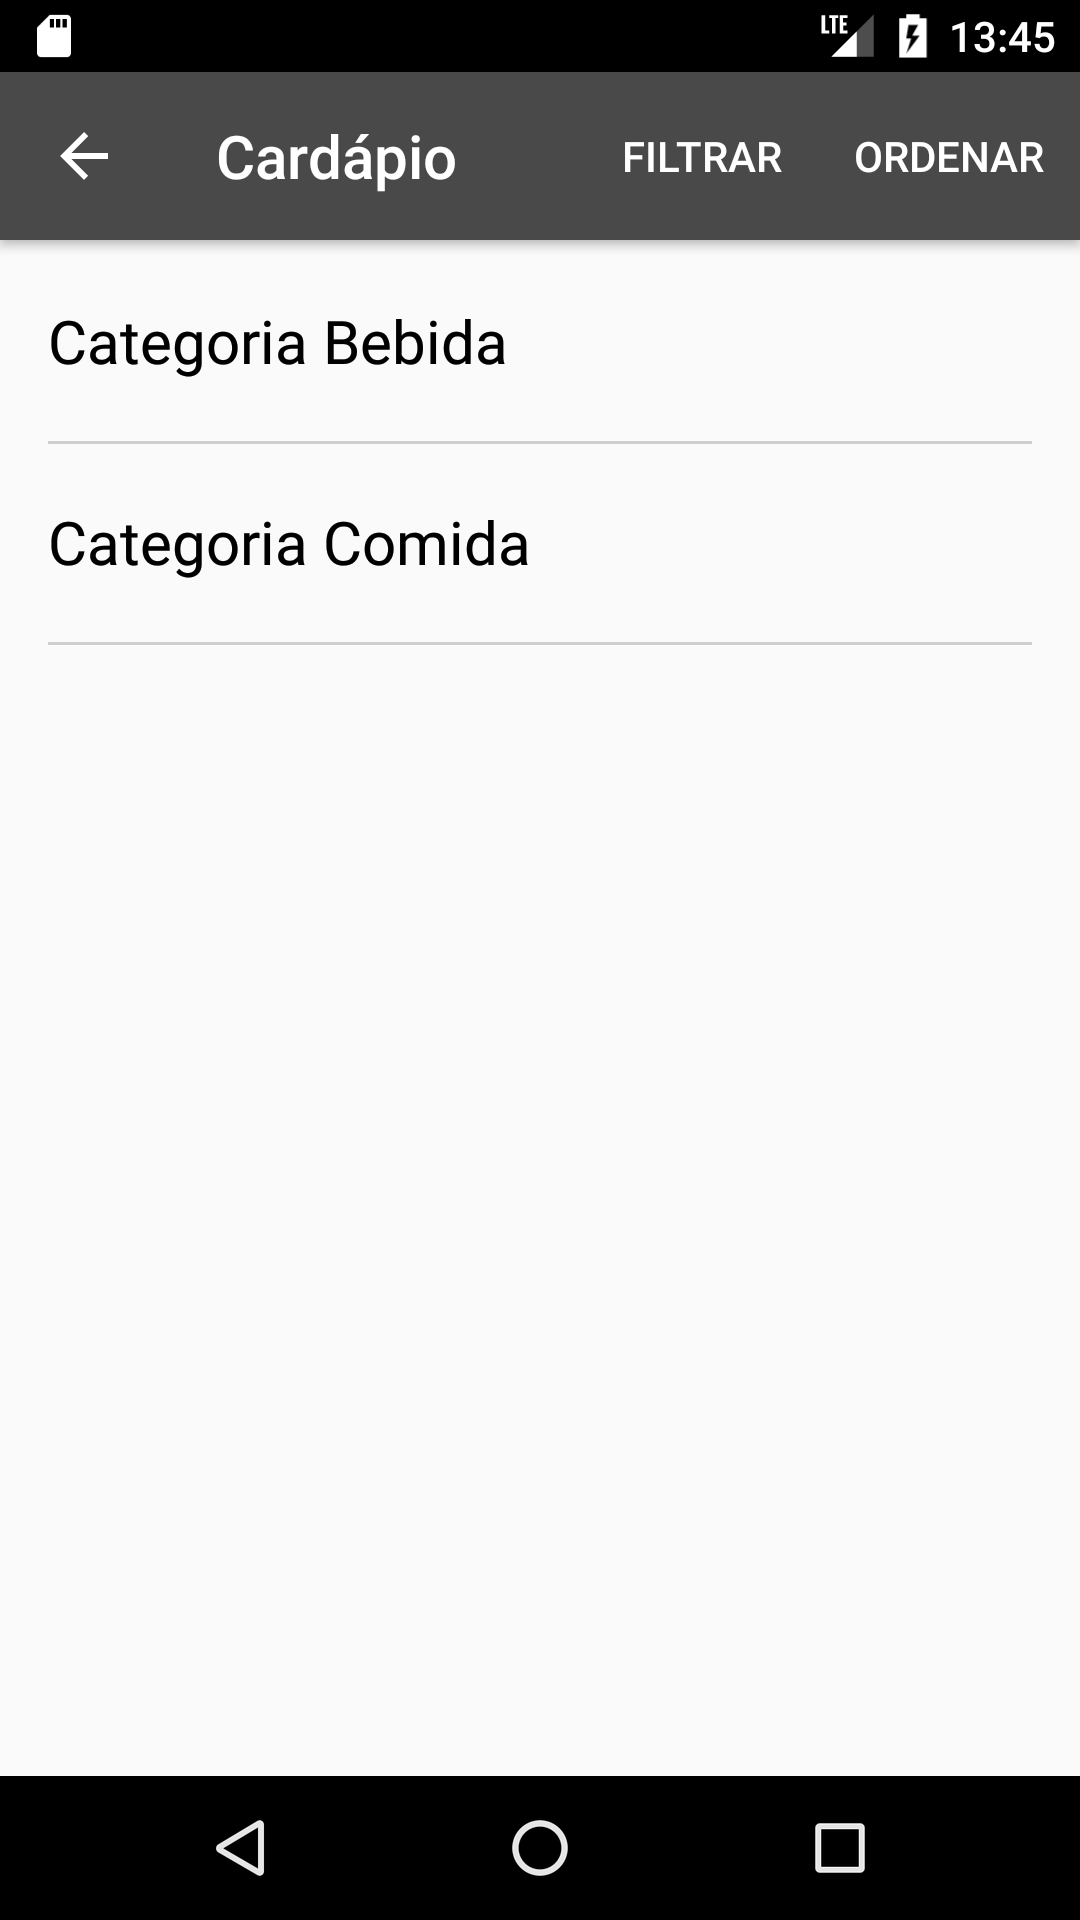
\includegraphics[width=0.3\textwidth]{./fig/cardapio-virtual/cardapio-1.png}}
	\qquad
	\subfigure[c][Tela de lanches do cardápio]
	{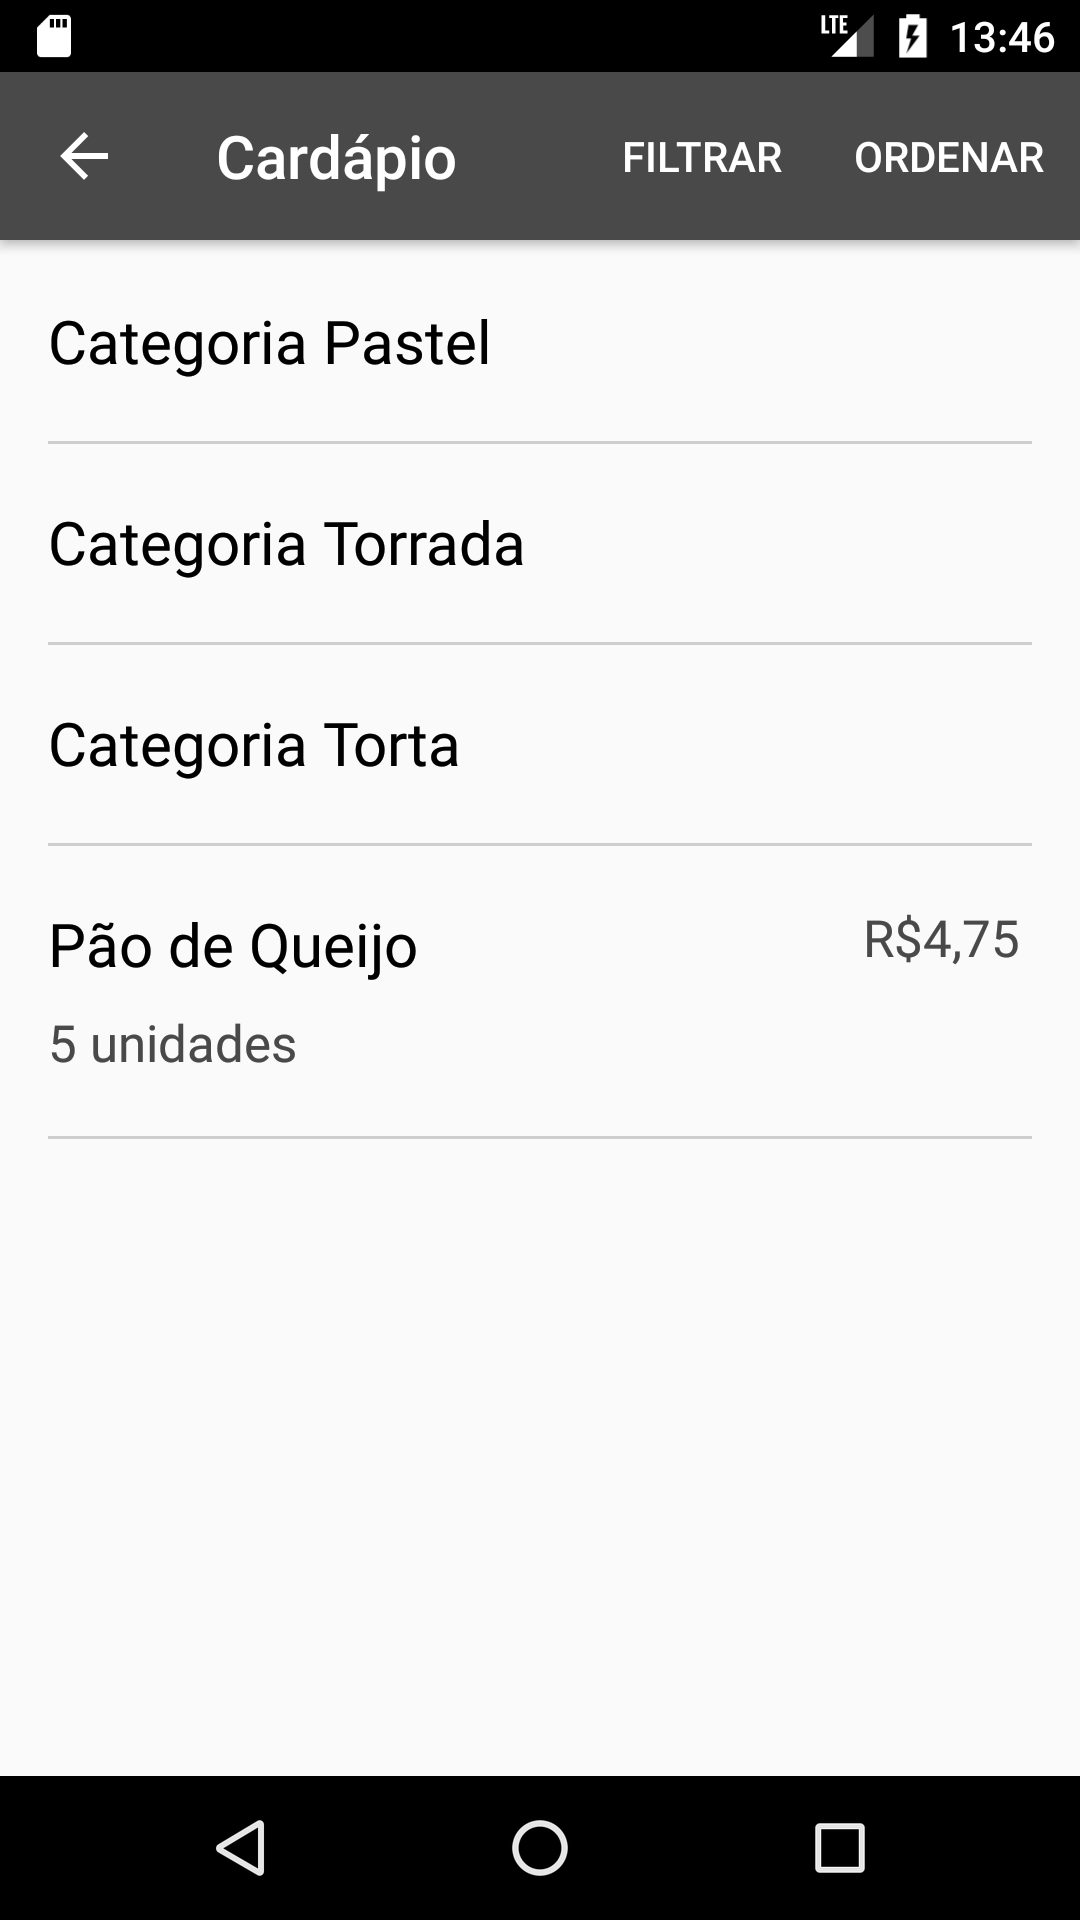
\includegraphics[width=0.3\textwidth]{./fig/cardapio-virtual/cardapio-2.png}}
	\qquad
	\subfigure[c][Filtros do cardápio]
	{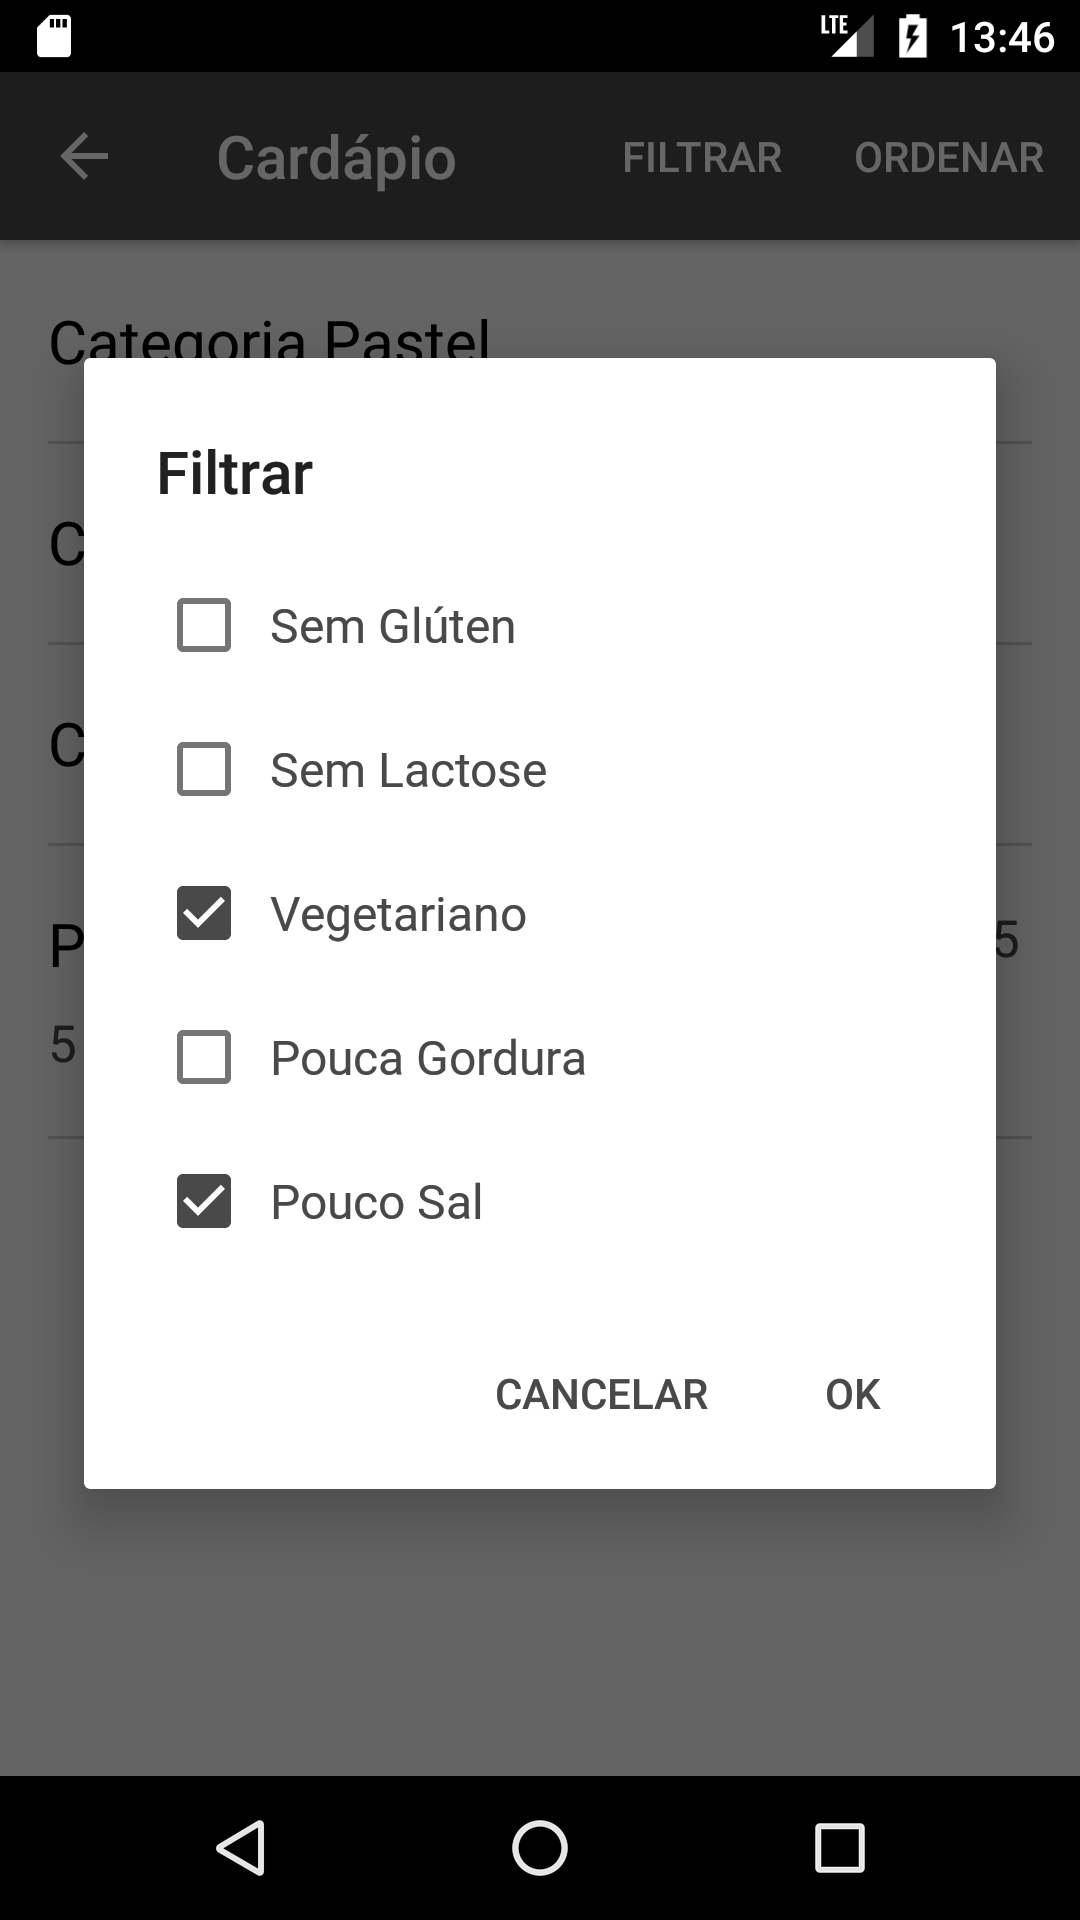
\includegraphics[width=0.3\textwidth]{./fig/cardapio-virtual/filtrar-1.png}}
	\qquad
	\subfigure[c][Ordenação do cardápio]
	{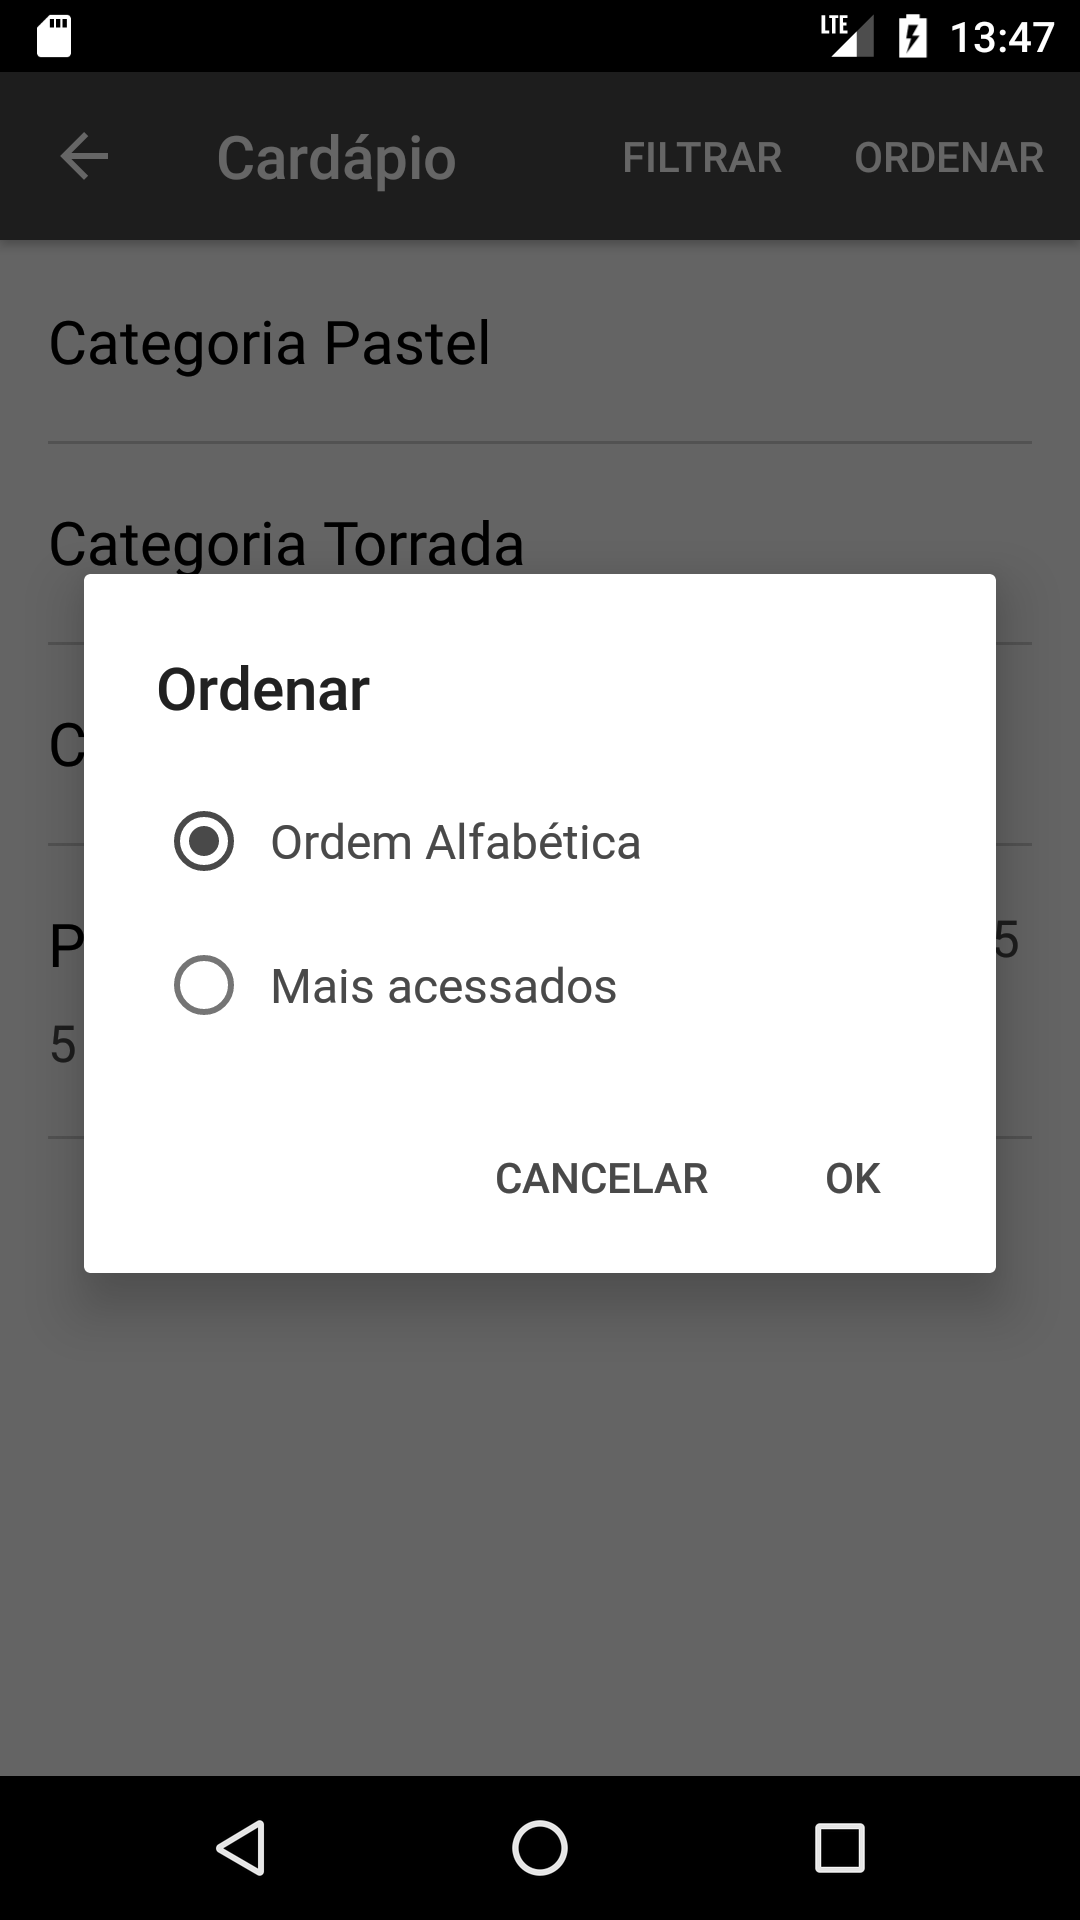
\includegraphics[width=0.3\textwidth]{./fig/cardapio-virtual/ordenar-1.png}}
\end{figure}

\begin{figure}[H] \ContinuedFloat
	\centering
	\caption[]{Continuação da página anterior}
	\label{fig:cardapio-virtual-4}
	\subfigure[c][Informações adicionais do produto]
	{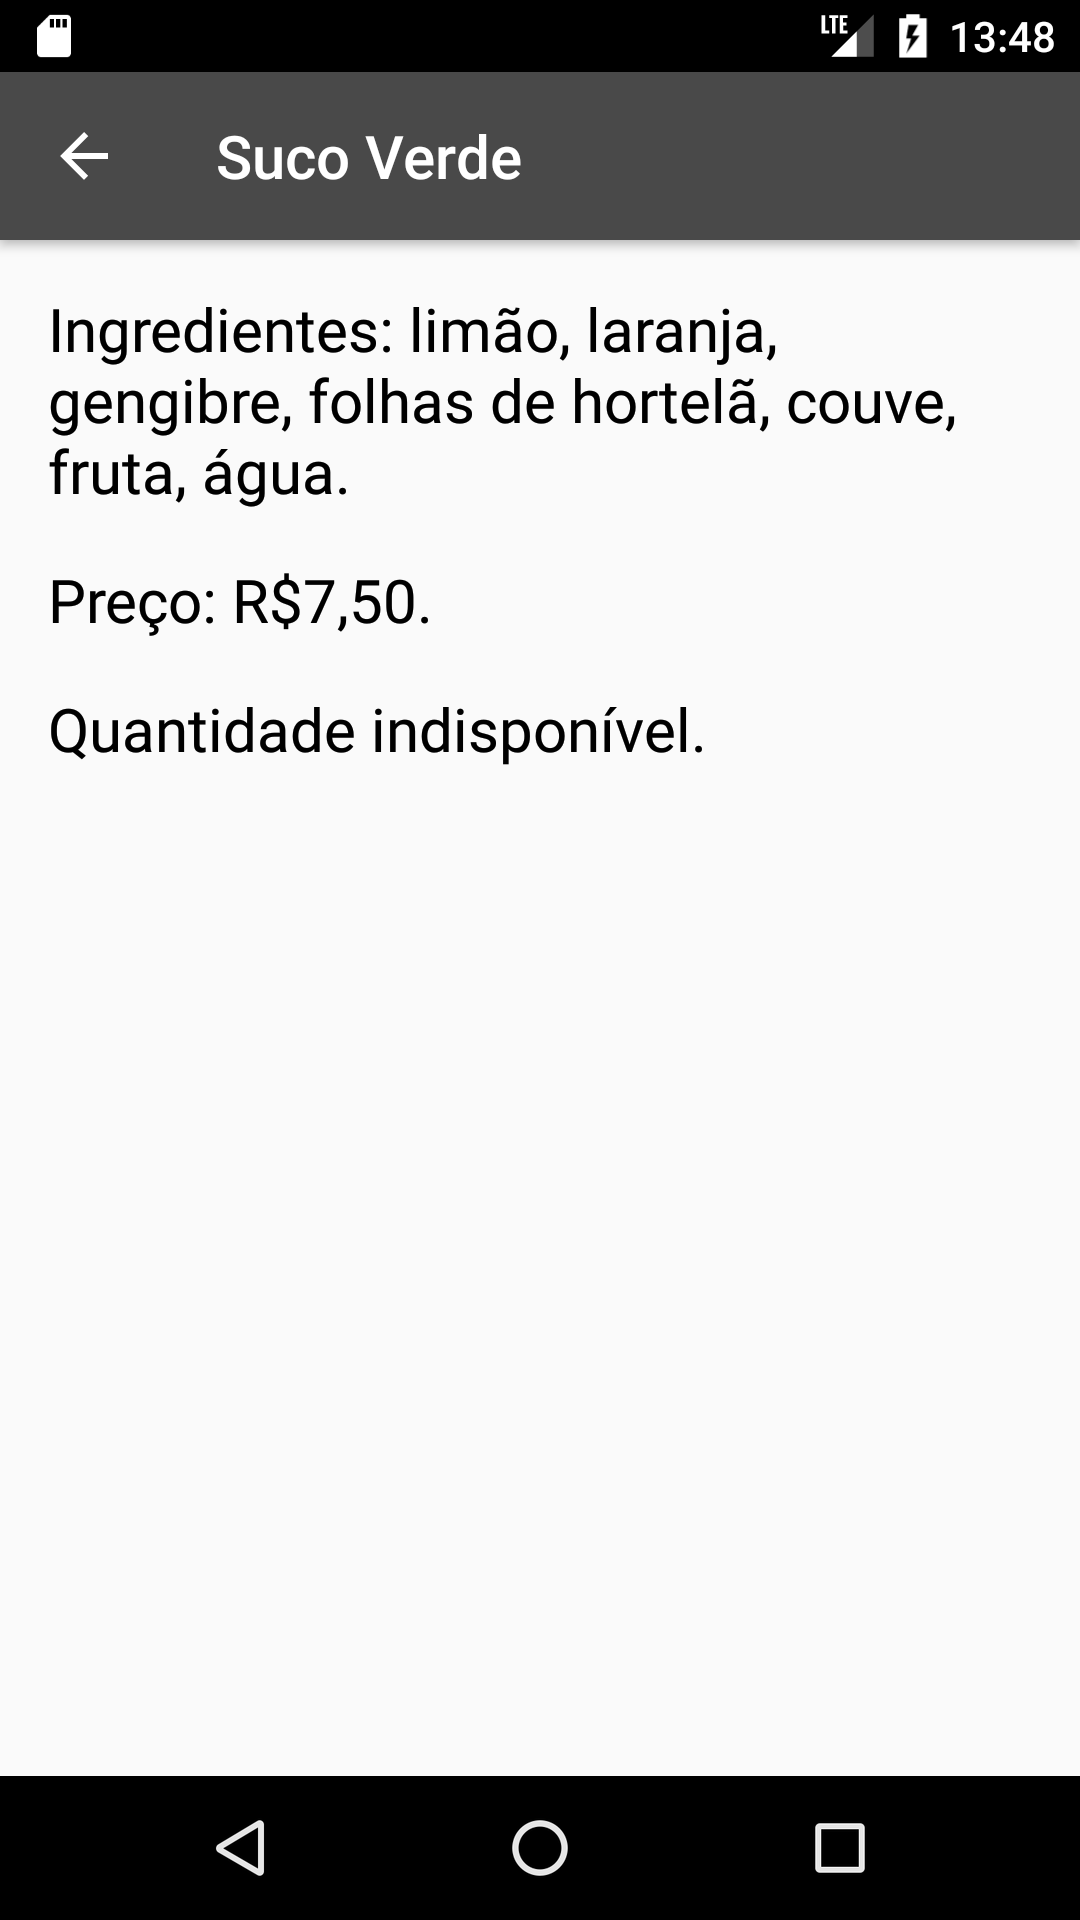
\includegraphics[width=0.3\textwidth]{./fig/cardapio-virtual/produto-1.png}}
\end{figure}
